\documentclass[12pt]{article}%
\usepackage[brazilian]{babel}
\usepackage[utf8]{inputenc}
\usepackage[T1]{fontenc}
\usepackage[a4paper, top=2.5cm, bottom=2.5cm, left=2.2cm, right=2.2cm]%
{geometry}
\usepackage{enumitem}
\usepackage{mathtools}
\usepackage{amsmath}
\usepackage{hyperref}
\usepackage{indentfirst}
\usepackage{graphicx}%
\usepackage{titling}
\usepackage{subfig}
\usepackage{tikz}
\usepackage{fancyhdr}
\usepackage{tikz}
\usepackage{systeme,mathtools}
\usepackage{minted}
\usepackage{mathtools}
\usepackage{empheq}
\usepackage{subcaption}
\usepackage{lipsum}% Just for this example
\usepackage{graphicx}
\usepackage{amsmath}

\setlist{  
  listparindent=\parindent,
  parsep=0pt,
}

\DeclarePairedDelimiter\abs{\lvert}{\rvert}%

\newcommand{\subtitle}[1]{%
  \posttitle{%
    \par\end{center}
    \begin{center}\large#1\end{center}
    \vskip0.5em}%
}
\newcommand{\newpara}
    {
    \vskip 0.5cm
    }

\newcommand{\newparaa}
    {
    \vskip 0.1cm
    }


\begin{document}
\begin{titlepage}
\begin{figure}[t]
\centering
\includegraphics[scale=0.6]{images/ufpe3.png}
\label{fig_ufpe}
\end{figure}
\begin{center} 
{\large Victor Miguel de Morais Costa (vmmc2)}\\[0.2cm]
{\large Victor Hugo Meirelles Silva (vhms)}\\[0.2cm]
{\large Zênio Ângelo Oliveira Neves (zaon)}\\[0.2cm]
{\large Zilde Souto Maior Neto (zsmn)}\\[5.5cm]
{\bf \Large RELATÓRIO DE PROJETO}\\[0.2cm]
{\large Métodos Numéricos}\\[5.5cm]
{\large Recife}\\[0.1cm]
{\large 2019}
\end{center}
\end{titlepage}

\thispagestyle{empty}
\pagebreak
\thispagestyle{empty}
\tableofcontents
\newpage    
\setcounter{page}{1}

\section{Introdução}

\newpage
\section{Primeiro Problema}
    Considere os dois tanques mostrados na figura. O tanque A possui 50 Litros de água no qual 25
    kilogramas de sal são dissolvidos. Suponha que o tanque B contenha 50 Litros de água pura inicialmente
    e que o liquido é bombeado para dentro e para fora dos tanques como mostrado na figura. A mistura
    trocada entre os dois tanques e o líquido bombeado para fora do tanque B são assumidos como estando
    bem misturados.
    \newpara
    \begin{center}
        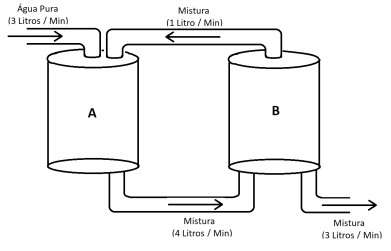
\includegraphics[scale=1.0]{problemas/p1.png}
    \end{center}
    
    (a) Construa um modelo matemático que descreva o número de quilogramas x1(t) e x2(t) de sal nos tanques A e B, respectivamente, no tempo t.
    \newpara
    (b) Usando os métodos numéricos implementados da primeira parte do projeto e a solução encontrada no quesito anterior, plote os gráficos de x1(t) e x2(t) mostrando os resultados na apresentação final. Não esqueça de comparar a eficiência dos métodos e a precisão em comparação com a solução exata.
    \newpara
    (c) Comente o que acontece quando t tende para o infinito.
    
    \subsection{Modelagem}
    As variações na quantidade de sal são devidas somente aos fluxos de entrada e de saida do tanque. Mais precisamente a taxa de variação de sal no tanque, \(\frac{dQ}{dt}\), é igual a taxa segundo a qual o sal está entrando menos a taxa segundo a qual ele está saindo:
    
    \begin{equation}
        \frac{dQ}{dt} = taxa_{entrada} - taxa_{saida}
    \end{equation}
    
    A taxa de variação de sal no tanque A (\(\frac{dQ_{A}}{dt}\)) é dada por:
    
    \begin{equation}
        \frac{dQ_{A}}{dt} = \frac{1}{50}  Q_{B} - \frac{2}{25}  Q_{A}
    \end{equation}
    
    A taxa de variação de sal no tanque B (\(\frac{dQ_{B}}{dt}\)) é dada por:
    
    \begin{equation}
        \frac{dQ_{B}}{dt} = \frac{2}{25}  Q_{A} - \frac{2}{25}  Q_{B}
    \end{equation}

    \subsection{Solução Analítica}

    Dessa forma, temos o seguinte sistema de equações lineares:
    
    \begin{empheq}[left=\empheqlbrace]{align}
      50Q'_{A} = Q_{B} - 4Q_{A} \\ 
      25Q'_{B} = 2Q_{A} - 2Q_{B}
    \end{empheq}
    
    Onde, aplicando Laplace para a primeira equação:
    
    \[50\mathcal{L}{Q'_{A}} = \mathcal{L}{Q_{B}} - 4\mathcal{L}{Q_{A}}\]
    \[50[s\mathcal{L}{Q_{A}} - Q_{A}(0)] = \mathcal{L}{Q_{B}} - 4\mathcal{L}{Q_{A}}\]
    \[50[s\mathcal{L}{Q_{A}} - 25] = \mathcal{L}{Q_{B}} - 4\mathcal{L}{Q_{A}}\]
    \[50s\mathcal{L}{Q_{A}} - 1250 = \mathcal{L}{Q_{B}}- 4\mathcal{L}{Q_{A}}\]
    \[50s\mathcal{L}{Q_{A}} + 4\mathcal{L}{Q_{A}} = \mathcal{L}{Q_{B}} + 1250\]
    \[50sF_{A} + 4F_{A} = F_{B} + 1250\]
    \[F_{A}[50s + 4] = F_{B} + 1250\]
    \[F_{A} = \frac{F_{B} + 1250}{50s + 4}\]
    
    \newpara
    E aplicando Laplace para a segunda equação:
    
    \[25Q'_{B}  = 2Q_{A} - 2Q_{B}\]
    \[25\mathcal{L}{Q'_{B}} = 2\mathcal{L}{Q_{A}} - 2\mathcal{L}{Q_{B}}\]
    \[25[s\mathcal{L}{Q_{B}} - 0] = 2\mathcal{L}{Q_{A}} - 2\mathcal{L}{Q_{B}}\]
    \[25sF_{B} = 2F_{A} - 2F_{B}\]
    \[25sF_{B} + 2F_{B} = 2F_{A}\]
    
    \newpara
    Aplicando o \(F_{A}\) obtido na primeira equação na segunda:
    
    \[25sF_{B} + 2F_{B} = 2\frac{F_{B} + 1250}{50s + 4}\]
    \[(25sF_{B} + 2F_{B})(50s + 4) = 2F_{B} + 2500\]
    \[1250s^2F_{B} + 100sF_{B} + 100sF_{B} + 8F_{B} = 2F{B} + 2500\]
    \[1250s^2F_{B} + 200sF_{B} + 6F_{B} = 2500\]
    \[F_{B}(1250s^2 + 200s + 6) = 2500\]
    \[F_{B}1250(s^2 + \frac{4}{25}s + \frac{3}{625}) = 2500\]
    \[F_{B}(s^2 + \frac{4}{25}s + \frac{3}{625}) = 2\]
    \[F_{B}(s + \frac{1}{25})(s + \frac{3}{25}) = 2\]
    \[F_{B} = \frac{2}{(s + \frac{1}{25})(s + \frac{3}{25})}\]
    
    \newpara
    Substituindo \(F_{B}\) encontrado na equação para \(F_{A}\) encontrada:
    
    \[F_{A} = \frac{\frac{2}{(s + \frac{1}{25})(s + \frac{3}{25})} + 1250}{50s + 4}\]
    \[F_{A} = \frac{\frac{2}{s^2 + \frac{4}{25}s + \frac{3}{625}} + 1250}{50s + 4}\]
    \[F_{A} = \frac{\frac{2 + 1250(s^2 + \frac{4}{25}s + \frac{3}{625})}{s^2 + \frac{4}{25}s + \frac{3}{625}}}{50s + 4}\]
    \[F_{A} = \frac{2 + 1250s^2 + 200s + 6}{s^2 + \frac{4}{25}s + \frac{3}{625}} \frac{1}{50s + 4}\]
    \[F_{A} = \frac{2 + 1250s^2 + 200s + 6}{(s^2 + \frac{4}{25}s + \frac{3}{625})(50s + 4)}\]
    
    \newpara
    Finalmente, aplicando o Laplace inverso em \(F_{A}\) e \(F_{B}\), obtemos:
    
    \[\mathcal{L}^{-1}[F_{A}] = \frac{25}{2}e^{-(3t)/25}(e^{2t/25} + 1)\]
    \[\mathcal{L}^{-1}[F_{B}] = 25e^{-(3t)/25}(e^{2t/25} - 1)\]

    \newpage
    \subsection{Gráfico das soluções numéricas}
    \begin{figure}[H]
        \begin{center}
            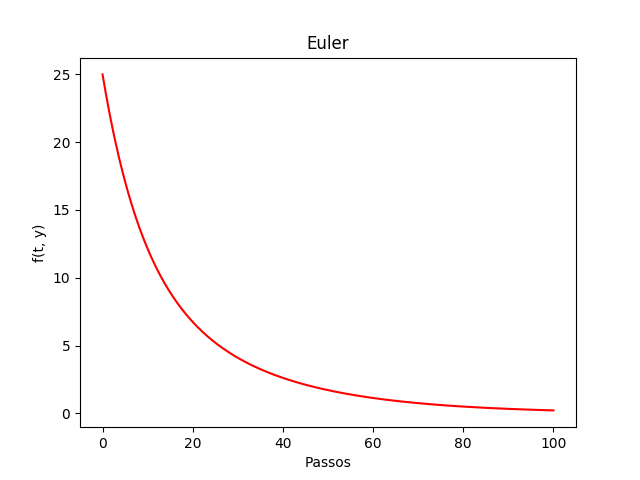
\includegraphics[width=.4\textwidth]{problemas/metodos_q1/tanque_a_euler.png}
            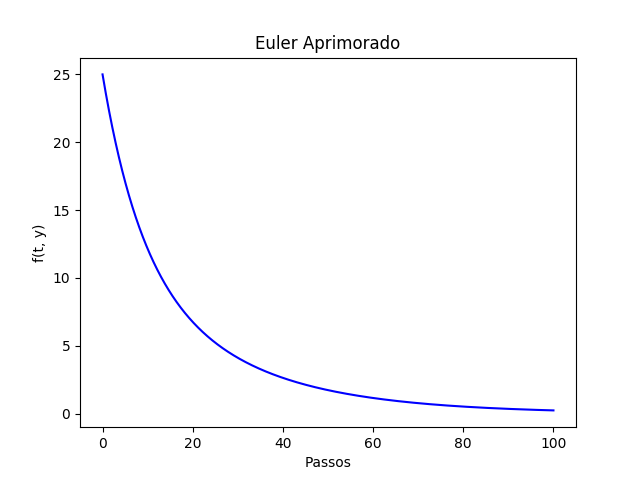
\includegraphics[width=.4\textwidth]{problemas/metodos_q1/tanque_a_euler_aprimorado.png}
            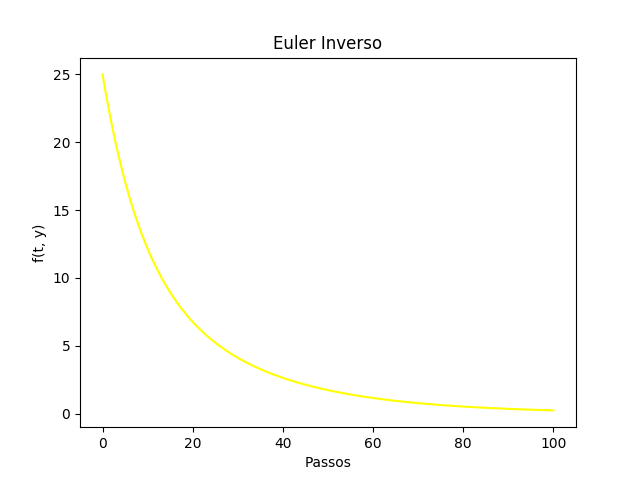
\includegraphics[width=.4\textwidth]{problemas/metodos_q1/tanque_a_euler_inverso.png}
            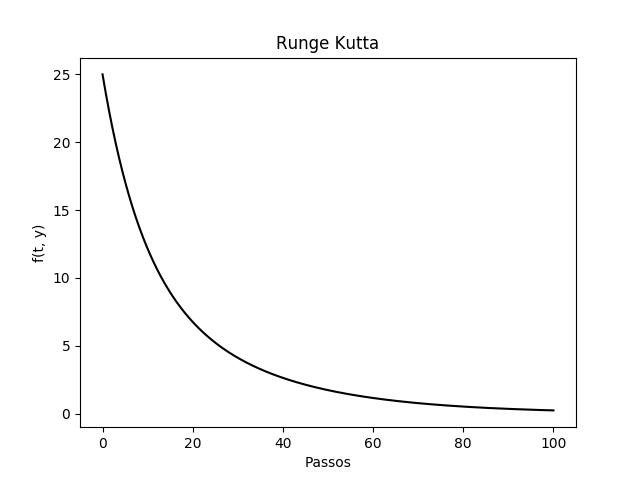
\includegraphics[width=.4\textwidth]{problemas/metodos_q1/tanque_a_runge_kutta.png}
        \end{center}
        \caption{Métodos de passos simples para a equação do tanque A}
    \end{figure}
    \begin{figure}[H]
        \begin{center}
            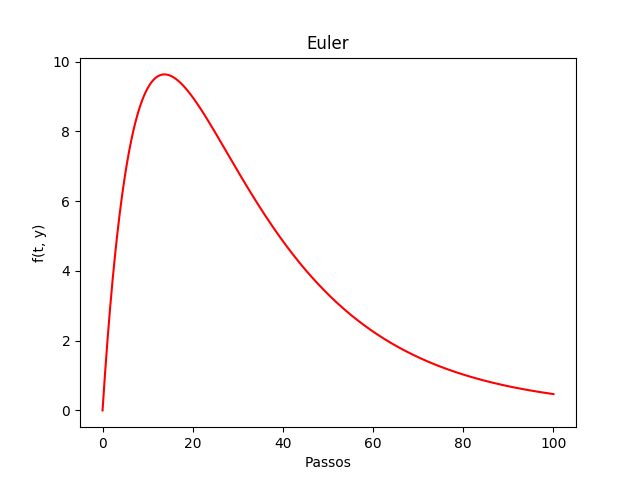
\includegraphics[width=.4\textwidth]{problemas/metodos_q1/tanque_b_euler.png}
            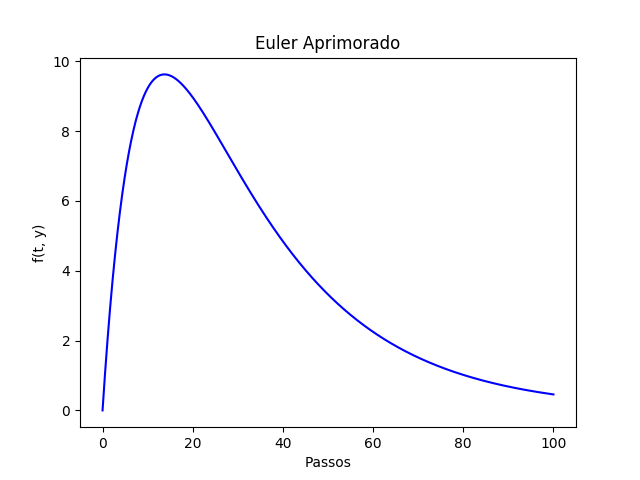
\includegraphics[width=.4\textwidth]{problemas/metodos_q1/tanque_b_euler_aprimorado.png}
            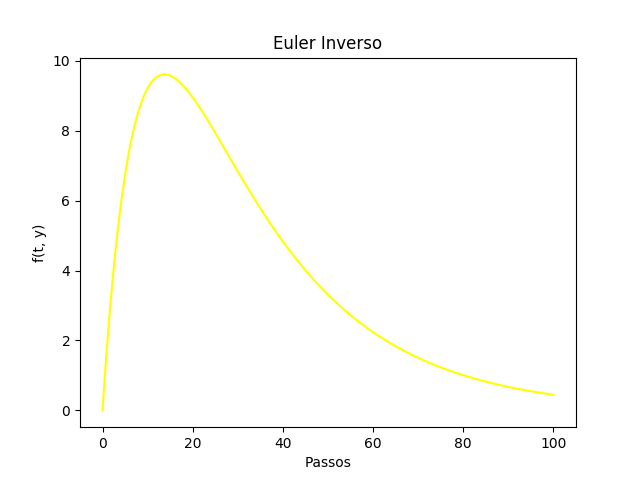
\includegraphics[width=.4\textwidth]{problemas/metodos_q1/tanque_b_euler_inverso.png}
            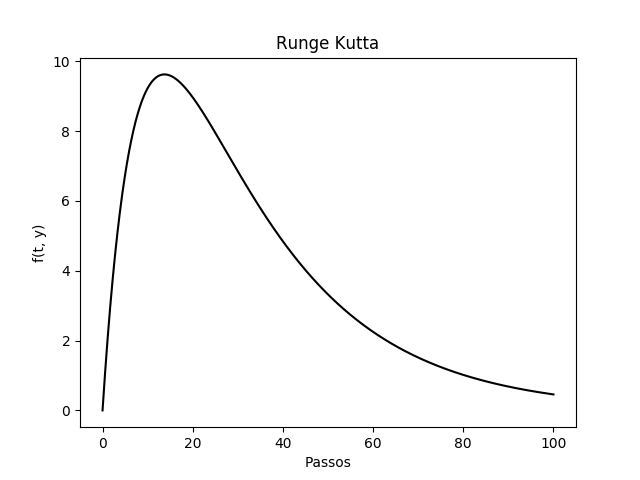
\includegraphics[width=.4\textwidth]{problemas/metodos_q1/tanque_b_runge_kutta.png}
        \end{center}
        \caption{Métodos de passos simples para a equação do tanque B}
    \end{figure}
    
    \begin{figure}[H]
        \begin{center}
            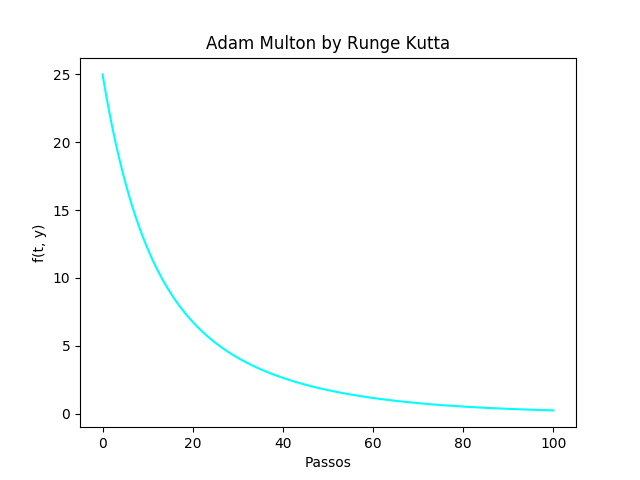
\includegraphics[width=.4\textwidth]{problemas/metodos_q1/tanque_a_multon.png}
            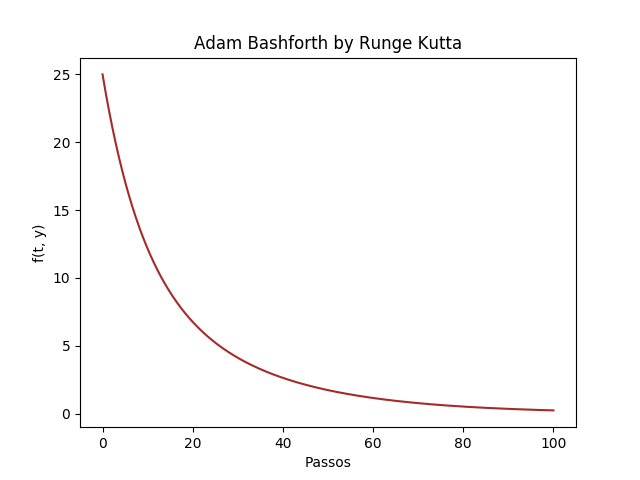
\includegraphics[width=.4\textwidth]{problemas/metodos_q1/tanque_a_bashforth.png}
            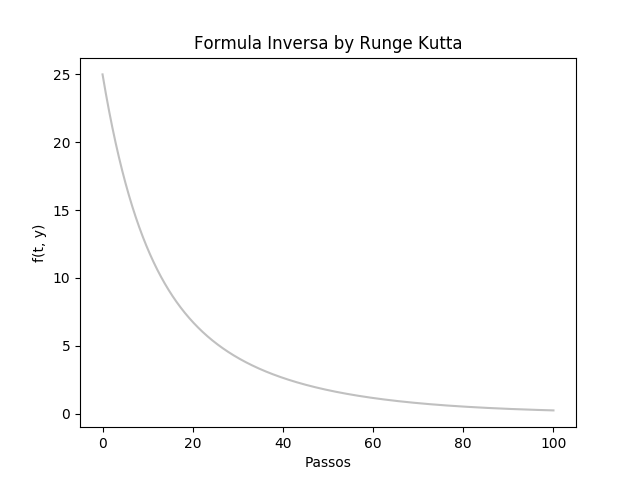
\includegraphics[width=.4\textwidth]{problemas/metodos_q1/tanque_a_inversa.png}
        \end{center}
        \caption{Métodos de passos múltiplos para a equação do tanque A}
    \end{figure}
    \begin{figure}[H]
        \begin{center}
            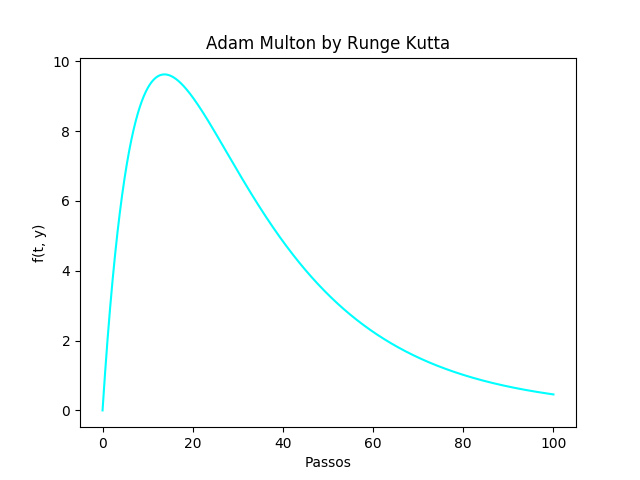
\includegraphics[width=.4\textwidth]{problemas/metodos_q1/tanque_b_multon.png}
            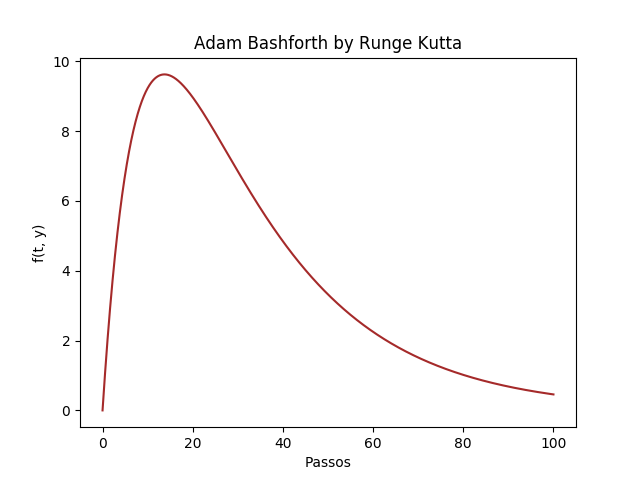
\includegraphics[width=.4\textwidth]{problemas/metodos_q1/tanque_b_bashforth.png}
            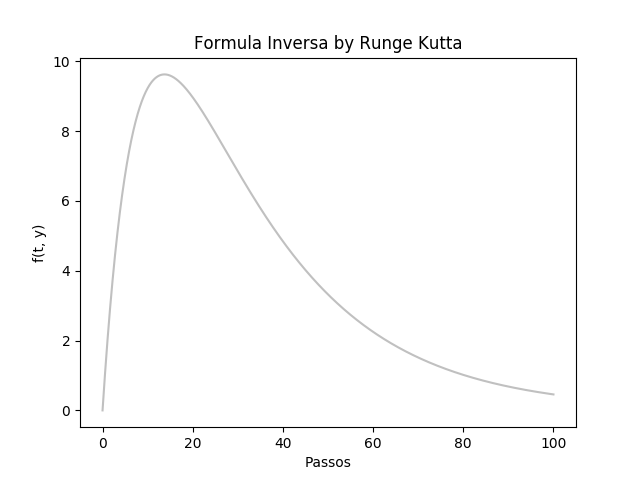
\includegraphics[width=.4\textwidth]{problemas/metodos_q1/tanque_b_inversa.png}
        \end{center}
        \caption{Métodos de passos múltiplos para a equação do tanque B}
    \end{figure}

    Como é possível notar nos gráficos gerados pelos métodos, tanto o tanque A quanto o tanque B tendem, após uma certa quantia de tempo, a uma cte. que pode ser calculada a partir do limite de suas equações quando t tender ao infinito:
    
    \[\lim_{t\to\infty} \frac{25}{2}e^{-(3t)/25}(e^{2t/25} + 1) = 0\]
    \[\lim_{t\to\infty} 25e^{-(3t)/25}(e^{2t/25} - 1) = 0\]
    
    Logo é possível notar que quando t tende ao infinito, ambas as equações que definem a quantidade de sal nos tanques tende a zero, ou seja, a água em ambos os tanques se torna totalmente pura.

    
\newpage
\section{Segundo Problema}
     (a) Descreva o sistema de equações diferenciais que descrevem \(i_{1}\)(t) e \(i_{2}\)(t) no circuito elétrico contendo um resistor, um indutor e um capacitor mostrado abaixo.

    \begin{center}
        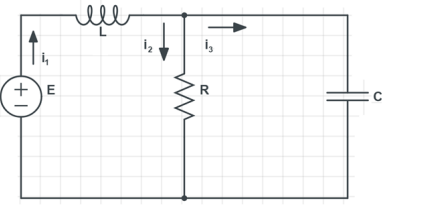
\includegraphics[scale=1.0]{problemas/p2a.png}
    \end{center}\
    
    (b) Resolva por Laplace o sistema encontrado supondo que \(E(t) = 60V, L = 1H, R = 50\Omega, C = 10^-4 F\) e que inicialmente \(i_{1} = i_{2} = 0\) (ver figura).

    \begin{center}
        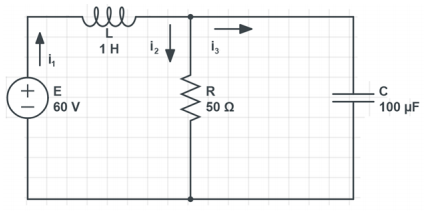
\includegraphics[scale=1.0]{problemas/p2b.png}
    \end{center}
    
    (c) Usando os métodos numéricos implementados da primeira parte do projeto e a solução exata
encontrada, plote os gráficos de i1(t) e i2(t) mostrando os resultados na apresentação e comparando a
eficiência dos métodos e as precisões em comparação com a solução exata. Comente o que acontece no
circuito quando t tende para infinito.

    \subsection{Modelagem}
    Pela lei das malhas, temos que a soma das diferenças de potenciais em uma malha é igual a zero, logo a partir da malha esquerda da figura temos:
    
    \begin{equation}
        E - L\frac{di_{1}}{dt} - i_{2}R = 0
        \label{p2_eq6}
    \end{equation}
    
    Já pela malha da direita da figura, temos:
    
    \begin{equation}
        \frac{Q}{C} - i_{2}R = 0
        \label{p2_eq7}
    \end{equation}
    
    Podemos escrever Q como a integral da corrente \(i_{3}\) em função do tempo:
    
    \begin{equation}
        \frac{1}{C} \int_{0}^{t} i_{3}tdt - i_{2}R = 0
        \label{p2_eq8}
    \end{equation}
    
    Resolvendo a integral da equação \ref{p2_eq8}, nós temos:
    
    \begin{equation}
        \frac{i_{3}t}{C} - i_{2}R = 0
        \label{p2_eq9}
    \end{equation}
    
    Por fim, derivando a equação \ref{p2_eq9} em relação ao tempo:
    
    \begin{equation}
        \frac{i_{3}}{C} - \frac{di_{2}}{dt} R = 0
        \label{p2_eq10}
    \end{equation}
    
    Pela regra da conservação das cargas, obtemos:
    
    \begin{equation}
        i_{1} = i_{2} + i_{3}
        \label{p2_eq11}
    \end{equation}
    
    Substituindo o valor de \(i_{3}\) obtido pela equação \ref{p2_eq11} na equação \ref{p2_eq10}, ficamos com:
    
    \begin{equation}
        \frac{i_{1} - i_{2}}{C} - \frac{di_{2}}{dt}R = 0
        \label{p2_eq12}
    \end{equation}
    
    Por fim, multiplicando a equação \ref{p2_eq12} por C, obtemos a seguinte equação:
    
    \begin{equation}
        i_{1} - i_{2} - RC\frac{di_{2}}{dt} = 0
        \label{p2_eq13}
    \end{equation}
    
    \subsection{Solução Analítica}
    
    Utilizando as equações \ref{p2_eq6} e \ref{p2_eq13} podemos formar o nosso sistema de equações:
    
    \begin{empheq}[left=\empheqlbrace]{align}
      E - L\frac{di_{1}}{dt} - i_{2}R &= 0 \\ 
      i_{1} - i_{2} - RC\frac{di_{2}}{dt} &= 0
    \end{empheq}
    
    Substituindo os valores informados no enunciado do problema nas equações \ref{p2_eq6} e \ref{p2_eq13} temos
    
    \begin{equation}
        60 - \frac{di_1}{dt} - 50i_2 = 0
    \label{p2_16}
    \end{equation}
    
    \begin{equation}
       i_1-i_2 - 5 \cdot 10^{-3}\frac{di_2}{dt} = 0
    \label{p2_17}
    \end{equation}
    
    Aplicando laplace na equação \ref{p2_16}, obtemos a seguinte equação:
    \begin{equation}
       \mathcal{L}{\frac{di_1}{dt}} = 60 \mathcal{L}{1}-50 \mathcal{L}{i_2}
    \label{p2_18}
    \end{equation}
    
    Usando as transformadas de Laplace, a equação \ref{p2_18} fica como: 
    \begin{equation}
      sI_1-i_1(0)=\frac{60}{s}-50I_2
    \label{p2_19}
    \end{equation}
    
    logo, reorganizando a equação:
    \begin{equation}
       I_1 = \frac{60}{s^2}-\frac{50I_2}{s} 
    \label{p2_20}
    \end{equation}
    
    Aplicando laplace na equação \ref{p2_17}, temos:
    
    \begin{equation}
      \mathcal{L}{i_1} = \mathcal{L}{i_2} + 5\cdot10^{-3} \mathcal{L}{\frac{di_2}{dt}}
    \label{p2_21}
    \end{equation}
    
    Usando as transformadas de Laplace, a equação \ref{p2_21} fica como:
    \begin{equation}
      I_1 = I_2 \cdot (1+5\cdot 10^{-3}s)
    \label{p2_22}
    \end{equation}
    
    Substituindo a equação \ref{p2_22} na equação \ref{p2_20} temos
    \begin{equation}
      I_2 \cdot (1 + 5 \cdot 10^{-3}s + \frac{50}{s}) = \frac{60}{s^2}
    \label{p2_23}
    \end{equation}
    
    Multiplicando ambos os lados da equação por s
    \begin{equation}
        I_2  (s + 5 \cdot 10^{-3}s^2 + 50s) = \frac{60}{s}
    \label{p2_24}
    \end{equation}
    
    Manipulando a equação \ref{p2_24} algebricamente
    \begin{equation}
      I_2 = \frac{120}{s(s^2+2s+100)}
    \label{p2_25}
    \end{equation}
    
    \begin{equation}
        I_2 = \frac{120}{s10^{-2}(s^2+2s+100)}
    \label{p2_26}
    \end{equation}
    
    \begin{equation}
        I_2 = \frac{12000}{s(s+100)^2}
    \label{p2_27}
    \end{equation}
    
    Usando a inversa de laplace na equação \ref{p2_27}
    \begin{equation}
      i_2(t) = 12\cdot10^3 \int_{0}^{t} \tau e^{-100\tau}\,d\tau
    \label{p2_28}
    \end{equation}
    
    E resolvendo a integral, encontramos o valor para $i_2$, segue
    \begin{equation}
      i_2(t) = \frac{1}{10000}[1 - (100t+1)e^{-100t}]\cdot 12 \cdot 10^3
    \label{p2_29}
    \end{equation}
    
    \begin{equation}
      i_2(t) = -120te^{-100t}-1.2e^{-100t}+1.2
    \label{p2_30}
    \end{equation}
    
    Substituindo a equação \ref{p2_27} na equação \ref{p2_22}, vemos que $I_1$ é 
    \begin{equation}
      I_1 = \frac{12 \cdot 10^3}{s \cdot(s+100)^2} + \frac{60}{(s+100)^2}
    \label{p2_31}
    \end{equation}
    
    Aplicando a inversa de laplace na equação \ref{p2_31} e substituindo o valor de $i_2$ encontrado na equação \ref{p2_30}, obtem-se:
    \begin{equation}
      i_1(t) = -120te^{-100t} - 1.2e^{-100t} + 1.2 + 60te^{-100t}
    \label{p2_32}
    \end{equation}
    
    portanto, reorganizando a equação:
    \begin{equation}
      i_1(t) = -60te^{-100t}-1.2e^{-100t} + 1.2
    \label{p2_33}
    \end{equation}
    
    Logo a solução por Laplace para o sistema encontrado na seção anterior e utilizando os valores informados no enunciado do problema é mostrada nas equações \ref{p2_30} e \ref{p2_33}.
    
    \newpage
    \subsection{Gráfico das soluções numéricas}
    \begin{figure}[H]
        \begin{center}
            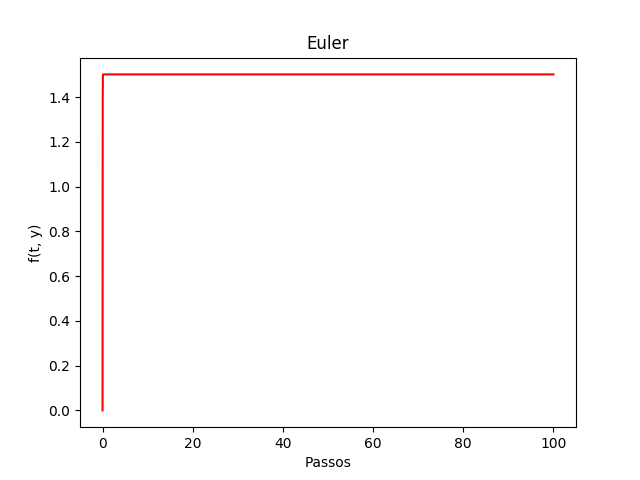
\includegraphics[width=.4\textwidth]{problemas/metodos_q2/circuito_euler.png}
            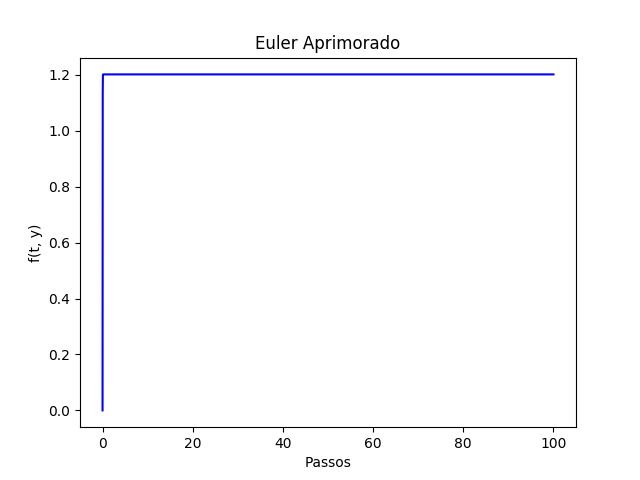
\includegraphics[width=.4\textwidth]{problemas/metodos_q2/circuito_euler_aprimorado.png}
            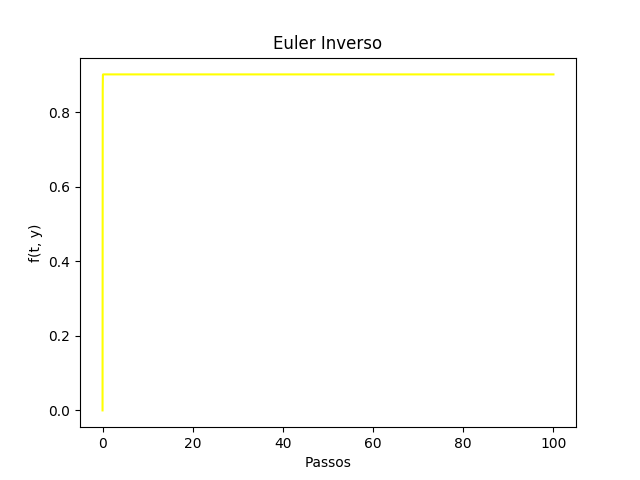
\includegraphics[width=.4\textwidth]{problemas/metodos_q2/circuito_euler_inverso.png}
            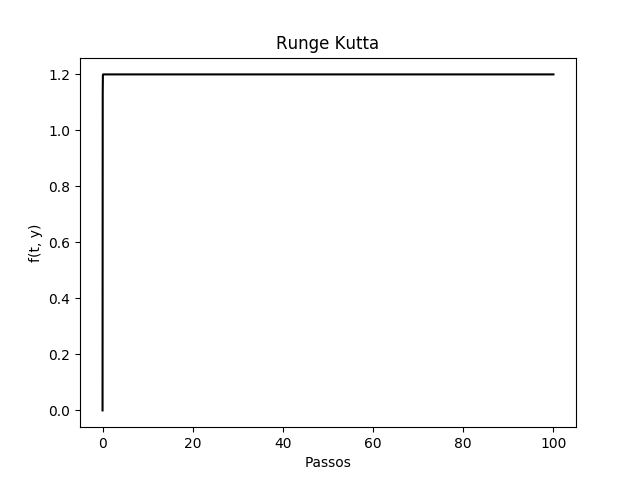
\includegraphics[width=.4\textwidth]{problemas/metodos_q2/circuito_runge_kutta.png}
        \end{center}
        \caption{Métodos de passos simples para a equação da corrente i1}
    \end{figure}
    \begin{figure}[H]
        \begin{center}
            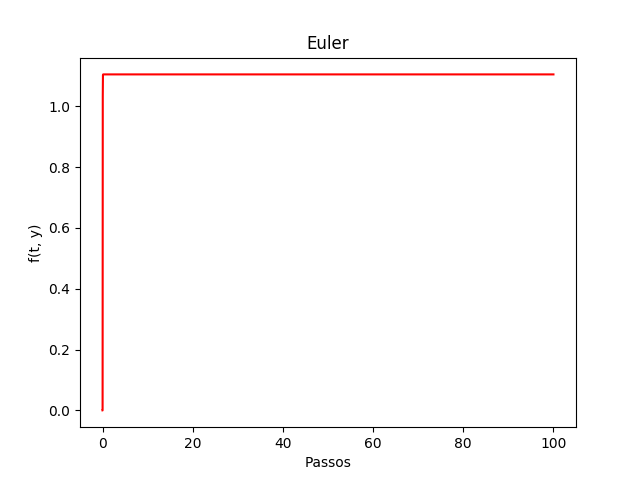
\includegraphics[width=.4\textwidth]{problemas/metodos_q2/circuito2_euler.png}
            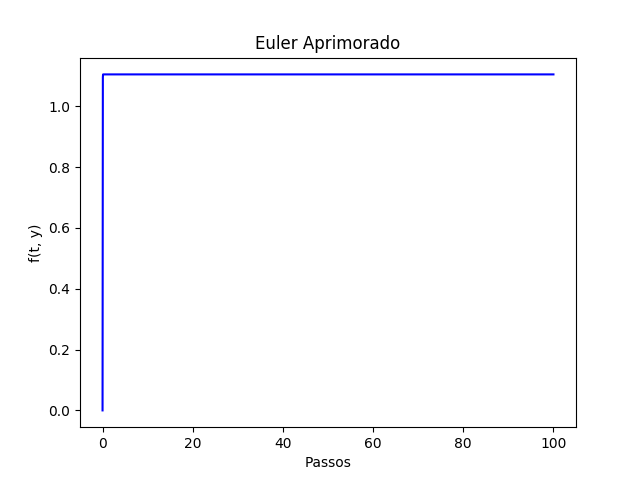
\includegraphics[width=.4\textwidth]{problemas/metodos_q2/circuito2_euler_aprimorado.png}
            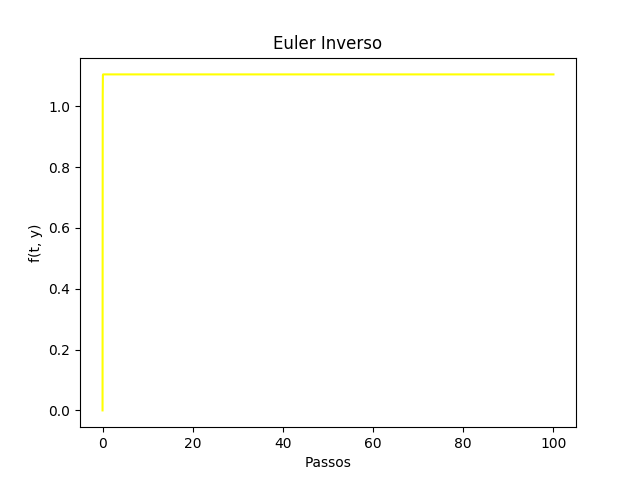
\includegraphics[width=.4\textwidth]{problemas/metodos_q2/circuito2_euler_inverso.png}
            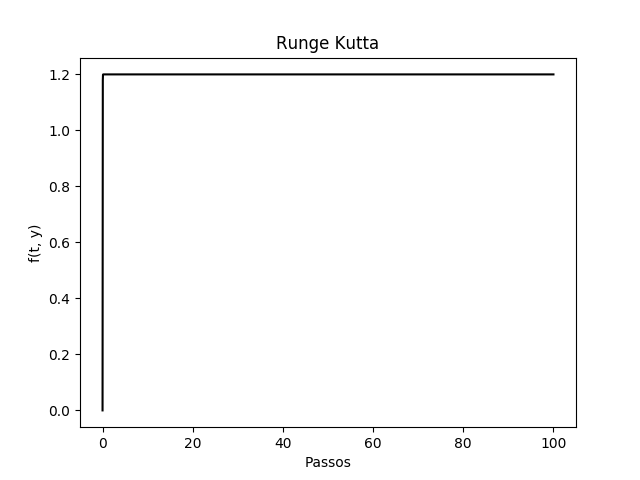
\includegraphics[width=.4\textwidth]{problemas/metodos_q2/circuito2_runge_kutta.png}
        \end{center}
        \caption{Métodos de passos simples para a equação da corrente i2}
    \end{figure}
    
    \begin{figure}[H]
        \begin{center}
            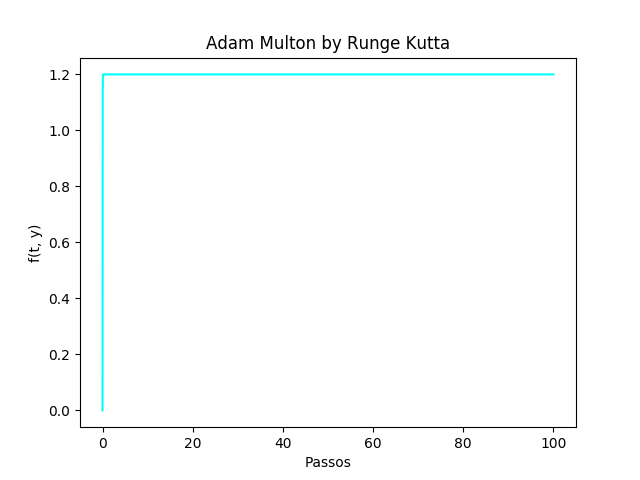
\includegraphics[width=.4\textwidth]{problemas/metodos_q2/circuito_multon.png}
            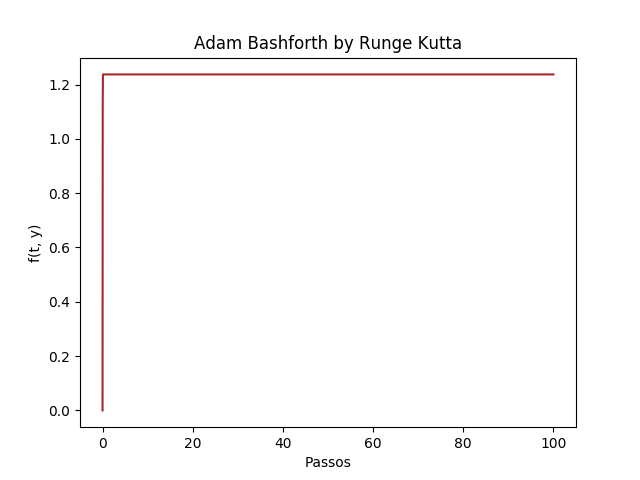
\includegraphics[width=.4\textwidth]{problemas/metodos_q2/circuito_bashforth.png}
            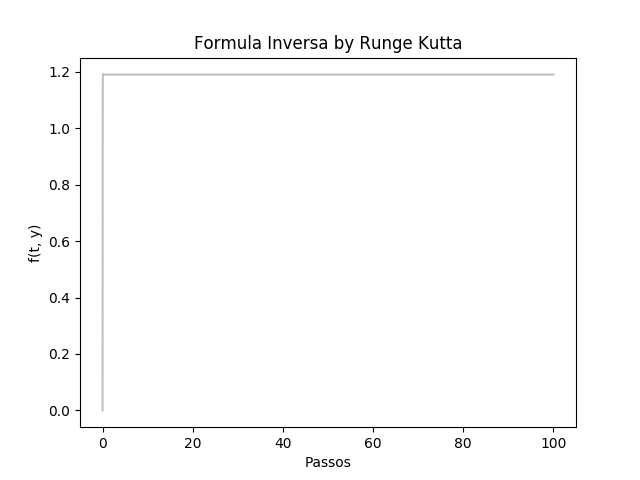
\includegraphics[width=.4\textwidth]{problemas/metodos_q2/circuito_inversa.png}
        \end{center}
        \caption{Métodos de passos simples para a equação da corrente i1}
    \end{figure}
    \begin{figure}[H]
        \begin{center}
            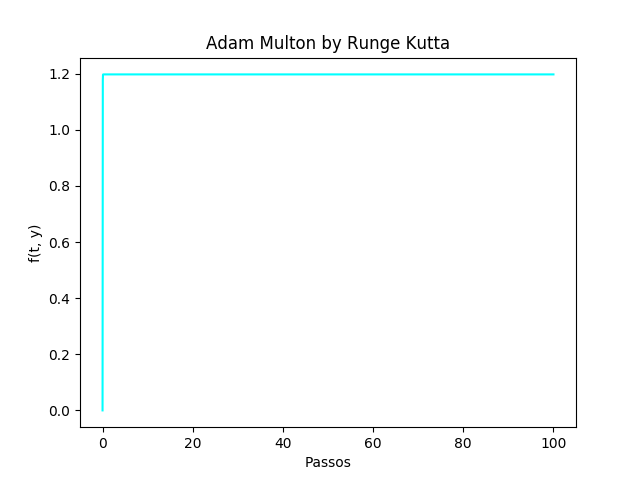
\includegraphics[width=.4\textwidth]{problemas/metodos_q2/circuito2_multon.png}
            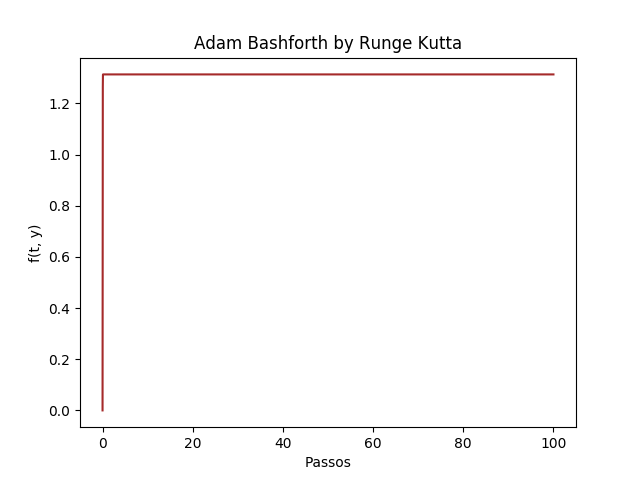
\includegraphics[width=.4\textwidth]{problemas/metodos_q2/circuito2_bashforth.png}
            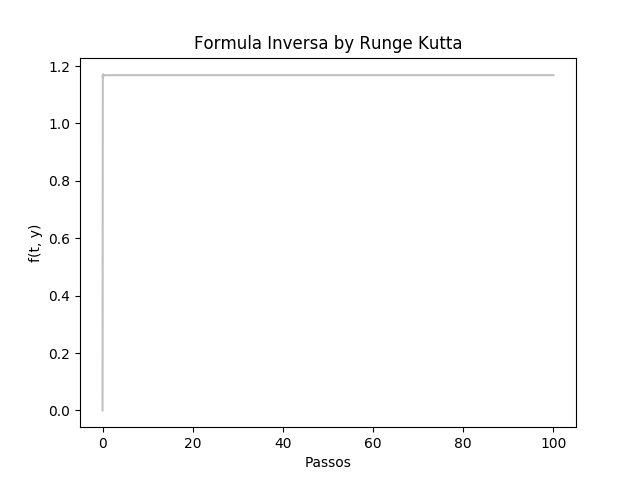
\includegraphics[width=.4\textwidth]{problemas/metodos_q2/circuito2_inversa.png}
        \end{center}
        \caption{Métodos de passos simples para a equação da corrente i2}
    \end{figure}
    
    Como é possível notar nos gráficos gerados pelos métodos, tanto a corrente i1 quanto a corrente i2 tendem, após uma certa quantia de tempo, a uma cte. que pode ser calculada a partir do limite de suas equações quando t tender ao infinito:
    
    \[\lim_{t\to\infty} i_{1}(t) = \lim_{t\to\infty} -60te^{-100t}-1.2e^{-100t} + 1.2 = 1.2\]
    \[\lim_{t\to\infty} i_{2}(t) = \lim_{t\to\infty} -120te^{-100t}-1.2e^{-100t} + 1.2 = 1.2\]
    
    Aplicando L'hospital em ambos os termos \(te^{-100t}\) nós notamos que nessa parcela de equação tende a zero, assim como no termo \(1.2e^{-100t}\) também temos tendência a zero, dessa forma o nosso limite fica como sendo o limite de uma constante (que é a própria constante), assumindo o valor de \(1.2\).
    
\newpage
\section{Terceiro Problema}
    (a) Descreva o sistema de equações diferenciais que descrevem i1(t) e i2(t) no circuito elétrico contendo dois resistores e dois indutores mostrado abaixo.

    \begin{center}
        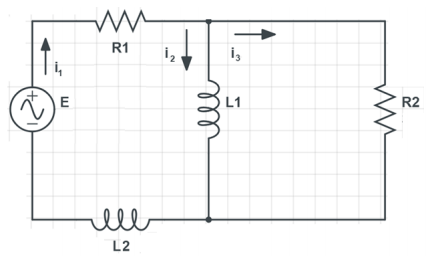
\includegraphics[scale=1.0]{problemas/p3a.png}
    \end{center}\
    
    (b) Use Variação dos paramêtros para resolver o sistema encontrado se, \(R1 = 8 \Omega, R2 = 3 \Omega, L1 = 1H, L2 = 1 H, E(t) = 100 sin(t)V, i1(0) = 0, i2(0) = 0\).

    \begin{center}
        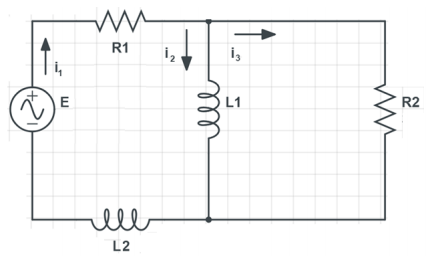
\includegraphics[scale=1.0]{problemas/p3b.png}
    \end{center}
    
    (c) Usando os métodos númericos implementados da primeira parte do projeto e a solução exata
encontrada, plote os gráficos de i1(t) e i2(t) mostrando os resultados na apresentação e comparando a
eficiencia dos métodos e a precisão em comparação com a solução exata. Comente qual o valor maximo
e minimo que a corrente pode atingir.

    \subsection{Modelagem}
    Pela lei das malhas, temos que a soma das diferenças de potenciais em uma malha é igual a zero, logo a partir da malha esquerda da figura temos:
    
    \begin{equation}
        -i_{1}R_{2} + i_{2}R_{2} - L_{2}i'_{1} + E - i_{1}R_{1} = 0
        \label{p3_eq34}
    \end{equation}
    
    Já usando a malha externa da figura, temos:
    
    \begin{equation}
        E = i_{3}R_{2} + L_{2}i'_{1} + i_{1}R_{1}
        \label{p3_eq35}
    \end{equation}
    
    Usando a lei dos nós de Kirchoff, também obtemos a seguinte equação:
    
    \begin{equation}
        i_{1} = i_{2} + i_{3}
        \label{p3_eq36}
    \end{equation}
    
    Dessa forma, podemos montar o seguinte sistema (já realizando as substituições de \ref{p3_eq36} em \ref{p3_eq35} e \ref{p3_eq34}:
    
    \begin{empheq}[left=\empheqlbrace]{align}
      E &= i_{1}R_{2} - i_{2}R_{2} + L_{2}i'_{1} + i_{1}R_{1} \\ 
      E &= i_{1}R_{1} + i'_{2}L_{1} + L_{2}i'_{1}
    \end{empheq}
    
    \subsection{Solução Analítica}
    
    Assumindo que A e B como a nossa primeira e a nossa segunda equação, respectivamente, podemos reescrever B como \(B = -B + A\)
    
    \begin{empheq}[left=\empheqlbrace]{align}
      E &= i_{1}R_{2} - i_{2}R_{2} + L_{2}i'_{1} + i_{1}R_{1} \\ 
      0 &= i_{1}R_{2} - i_{2}R_{2} - i'_{2}L_{1}
    \end{empheq}
    
    Dividindo A por \(L_{2}\) \((A = \frac{A}{L_{2}})\) e B por \(L_{1}\) \((B = \frac{B}{L_{1}})\), temos:
    
    \begin{empheq}[left=\empheqlbrace]{align}
      \frac{E}{L_{2}} &= \frac{i_{1}R_{2}}{L_{2}} - \frac{i_{2}R_{2}}{L_{2}} + i'_{1} + \frac{i_{1}R_{1}}{L_{2}} \\ 
      0 &= \frac{i_{1}R_{2}}{L_{1}} - \frac{i_{2}R_{2}}{L_{1}} - i'_{2}
    \end{empheq}
    
    Reescrevendo em forma de matriz, temos:
    
    \[
    \frac{d}{dt}
    \begin{bmatrix}
        i_{1}     \\
        i_{2}      
    \end{bmatrix}
    = 
    \begin{bmatrix}
        (\frac{-R_{1}}{L_{2}} - \frac{-R_{2}}{L_{2}})  &  \frac{R_{2}}{L_{2}}      \\
        \frac{R_{2}}{L_{1}}  &  \frac{-R_{2}}{L_{1}}      
    \end{bmatrix} 
    \cdot
    \begin{bmatrix}
        i_{1}     \\
        i_{2}      
    \end{bmatrix}
    +
    \begin{bmatrix}
        \frac{E}{L_{2}}     \\
        0      
    \end{bmatrix}
    \]
    
    Substituindo os valores do enunciado, temos que:
    
    \[
    \frac{d}{dt}
    \begin{bmatrix}
        i_{1}     \\
        i_{2}      
    \end{bmatrix}
    = 
    \begin{bmatrix}
       -11  &  3      \\
       3  &  -3     
    \end{bmatrix} 
    \cdot
    \begin{bmatrix}
        i_{1}     \\
        i_{2}      
    \end{bmatrix}
    +
    \begin{bmatrix}
        100\sin{t}     \\
        0      
    \end{bmatrix}
    \]
    
    Calculando o determinante, obtemos:
    
    \begin{equation}
        r^2 + 14r + 24 = 0
    \end{equation}
    
    Cujas raizes são:
    
    \begin{empheq}[left=\empheqlbrace]{align}
      r_{1} &= -2 \\ 
      r_{2} &= -12
    \end{empheq}
    
    Para a raiz \(r_{1} = -2\), obtem-se a seguinte matriz:
    
    \[
        \begin{bmatrix}
           -9  &  3      \\
           3  &  -1     
        \end{bmatrix} 
        \cdot
        \begin{bmatrix}
            \xi_{1}     \\
            \xi_{2}      
        \end{bmatrix}
        = 
        0
    \]
    
    De onde obtemos o seguinte sistema:
    
    \begin{empheq}[left=\empheqlbrace]{align}
      -9\xi_{1} + 3\xi_{2} &= 0
    \end{empheq}
    
    Logo, obtemos:
    
    \begin{equation}
        3\xi_{2} = 9\xi_{1}
    \end{equation}
    
    Portanto:
    
    \begin{equation}
        \xi_{2} = 3\xi_{1}
    \end{equation}
    
    Dessa forma, obtemos então:
    
    \[
        \xi^{1}
        =
        \begin{bmatrix}
            1 \\
            3
        \end{bmatrix}
    \]
    
    Para a raiz \(r_{1} = -12\), obtem-se a seguinte matriz:
    
    \[
        \begin{bmatrix}
           1  &  3      \\
           3  &  9     
        \end{bmatrix} 
        \cdot
        \begin{bmatrix}
            \xi_{1}     \\
            \xi_{2}      
        \end{bmatrix}
        = 
        0
    \]
    
    De onde obtemos o seguinte sistema:
    
    \begin{empheq}[left=\empheqlbrace]{align}
      \xi_{1} + 3\xi_{2} &= 0 \\
      3\xi_{1} + 9\xi_{2} &= 0
    \end{empheq}
    
    Logo, obtemos:
    
    \begin{equation}
        \xi_{1} = -3\xi_{2}
    \end{equation}
    
    Dessa forma, obtemos então:
    
    \[
        \xi^{2}
        =
        \begin{bmatrix}
            3 \\
            -1
        \end{bmatrix}
    \]
    
    Logo a equação homogênea é dada por:
    
    \begin{equation}
        x(t)_{H} = C_{1} 
        \begin{bmatrix}
            1 \\
            3
        \end{bmatrix}
        e^{-2t} + C_{2}
        \begin{bmatrix}
            3 \\
            -1
        \end{bmatrix}
        e^{-12t}
    \end{equation}
    
    Com isso, chegamos a matriz fundamental:
    
    \begin{equation}
        \Phi = 
        \begin{bmatrix}
            e^{-2t} & 3e^{-12t} \\
            3e^{-2t} & -e^{-12t} 
        \end{bmatrix}
    \end{equation}
    
    A partir da matriz fundamental podemos obter a matriz fundamental inversa:
    
    \begin{equation}
        \Phi^{-1} = \frac{1}{\abs{A}}
        \cdot 
        \begin{bmatrix}
            C_{11} & C_{21} \\
            C_{12} & C_{22}
        \end{bmatrix}
        =
        \begin{bmatrix}
            \frac{e^{2t}}{10} & \frac{3e^{2t}}{10} \\
            \frac{3e^{12t}}{10} & \frac{-e^{12t}}{10}
        \end{bmatrix}
    \end{equation}
    
    Dessa forma, como tinhamos a seguinte expressão:
    
    \[
    \frac{d}{dt}
    \begin{bmatrix}
        i_{1}     \\
        i_{2}      
    \end{bmatrix}
    = 
    \begin{bmatrix}
       -11  &  3      \\
       3  &  -3     
    \end{bmatrix} 
    \cdot
    \begin{bmatrix}
        i_{1}     \\
        i_{2}      
    \end{bmatrix}
    +
    \begin{bmatrix}
        100\sin{t}     \\
        0      
    \end{bmatrix}
    \]
    
    Podemos encontrar I' a partir da seguinte equação:
    
    \begin{equation}
        I' = AI + F(t)
    \end{equation}
    
    Temos que, pela definição:
    
    \begin{equation}
        I_{p} = \Phi \cdot U
        \label{p3_eq54}
    \end{equation}
    
    Podemos encontrar o valor de U a partir da seguinte equação:
    
    \begin{equation}
        U = \int \Phi^{-1} F(t) dt
        = 
        \int 
        \begin{bmatrix}
            10e^{2t}\sin{t} \\
            30e^{12t}\sin{t}
        \end{bmatrix}
        dt
    \end{equation}
    
    Logo, colocando o resultado na eq.\ref{p3_eq54}:
    
    \begin{equation}
        I_{p} = 
        \begin{bmatrix}
            \frac{332\sin{t}}{29} & \frac{-76\cos{t}}{29} \\
            \frac{276\sin{t}}{29} & \frac{-168\cos{t}}{29}
        \end{bmatrix}
    \end{equation}
    
    Logo, como em
    \(
        I(0) = 
        \begin{bmatrix}
            0 \\
            0
        \end{bmatrix}
    \) teremos, por fim, que as constantes \(C_{1}\) e \(C_{2}\) são:
    
    \begin{empheq}[left=\empheqlbrace]{align}
      C_{1} &= 2 \\
      C_{2} &= \frac{6}{29}
    \end{empheq}
    
    Logo, substituindo na homogênea encontrada, obtemos a solução geral:
    
    \begin{equation}
        \begin{bmatrix}
            i_{1} \\
            i_{2}
        \end{bmatrix}
        =
        2
        \cdot
        \begin{bmatrix}
            1 \\
            3
        \end{bmatrix}
        e^{-2t}
        +
        \frac{6}{29}
        \cdot
        \begin{bmatrix}
            3 \\
            -1
        \end{bmatrix}
        e^{-12t}
        +
        \begin{bmatrix}
            \frac{332\sin{t}}{29} & \frac{-76\cos{t}}{29} \\
            \frac{276\sin{t}}{29} & \frac{-168\cos{t}}{29}
        \end{bmatrix}
    \end{equation}
    
    \subsection{Gráfico das soluções numéricas}
    \begin{figure}[H]
        \begin{center}
            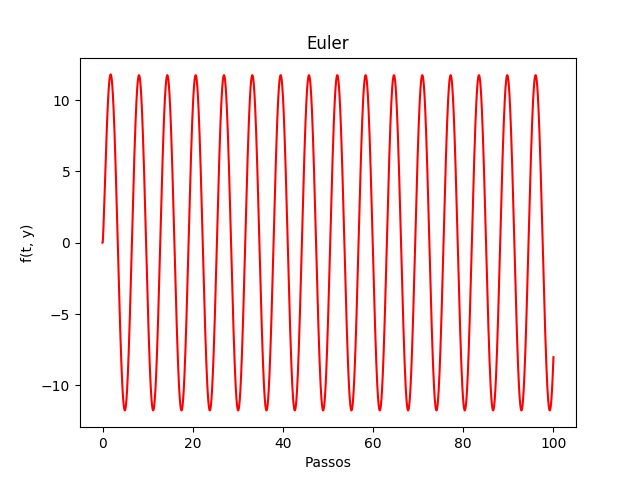
\includegraphics[width=.4\textwidth]{problemas/metodos_q3/circuito_euler.png}
            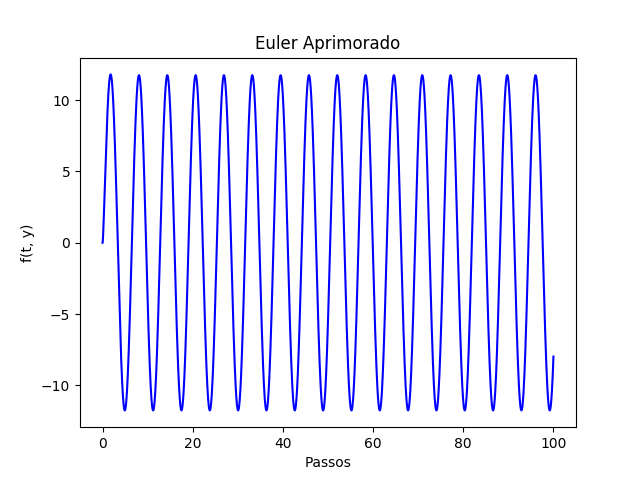
\includegraphics[width=.4\textwidth]{problemas/metodos_q3/circuito_euler_aprimorado.png}
            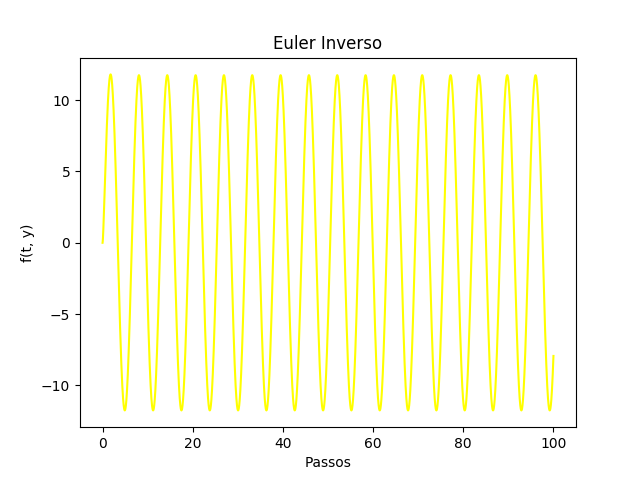
\includegraphics[width=.4\textwidth]{problemas/metodos_q3/circuito_euler_inverso.png}
            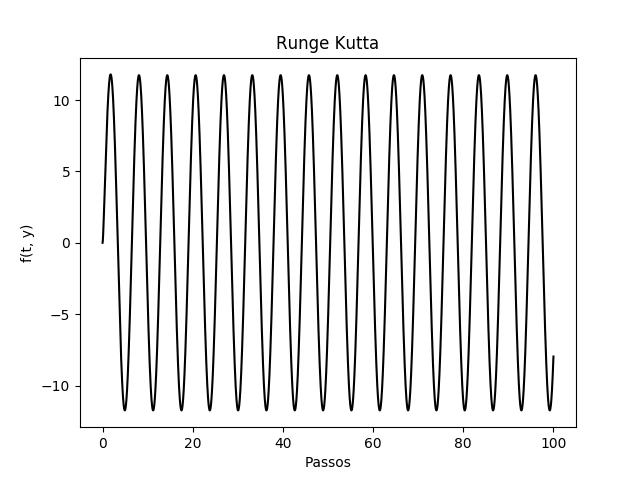
\includegraphics[width=.4\textwidth]{problemas/metodos_q3/circuito_runge_kutta.png}
        \end{center}
        \caption{Métodos de passos simples para a equação da corrente i1}
    \end{figure}
    \begin{figure}[H]
        \begin{center}
            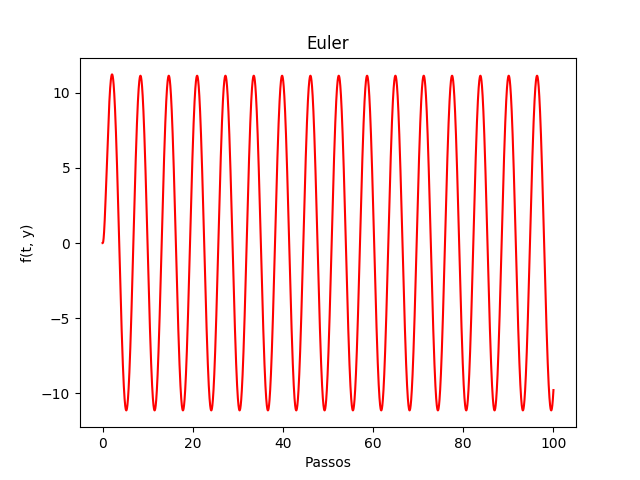
\includegraphics[width=.4\textwidth]{problemas/metodos_q3/circuito2_euler.png}
            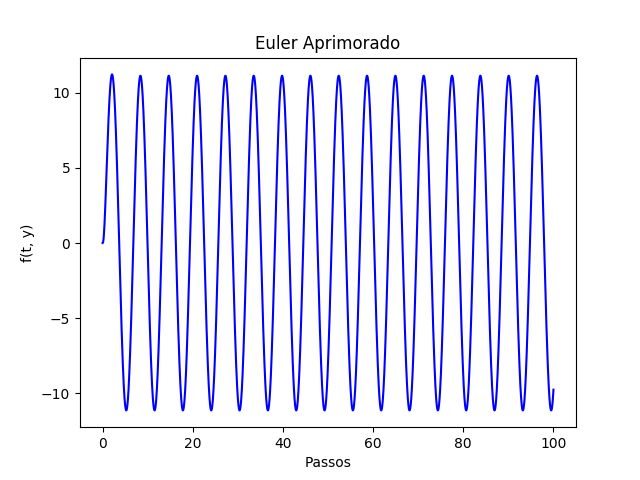
\includegraphics[width=.4\textwidth]{problemas/metodos_q3/circuito2_euler_aprimorado.png}
            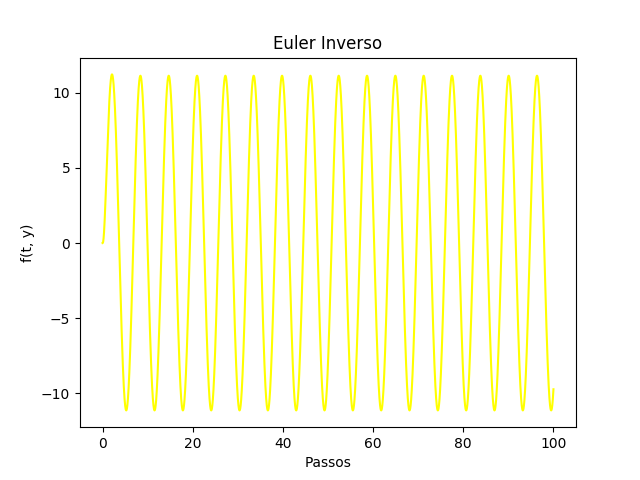
\includegraphics[width=.4\textwidth]{problemas/metodos_q3/circuito2_euler_inverso.png}
            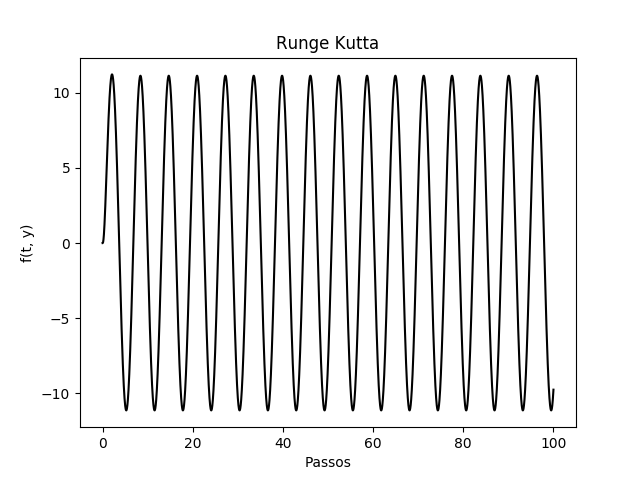
\includegraphics[width=.4\textwidth]{problemas/metodos_q3/circuito2_runge_kutta.png}
        \end{center}
        \caption{Métodos de passos simples para a equação da corrente i2}
    \end{figure}
    
    \begin{figure}[H]
        \begin{center}
            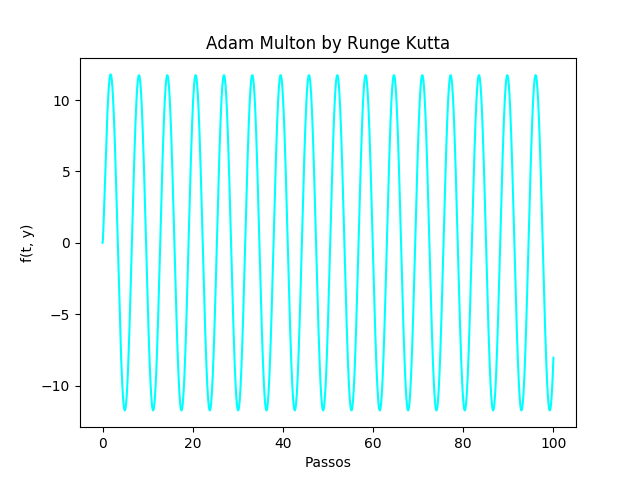
\includegraphics[width=.4\textwidth]{problemas/metodos_q3/circuito_multon.png}
            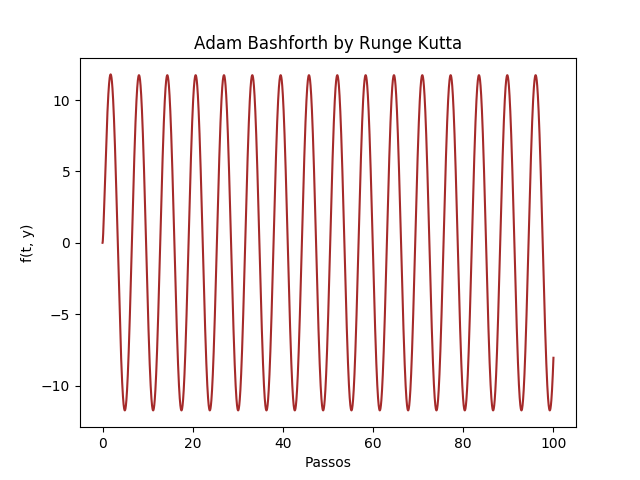
\includegraphics[width=.4\textwidth]{problemas/metodos_q3/circuito_bashforth.png}
            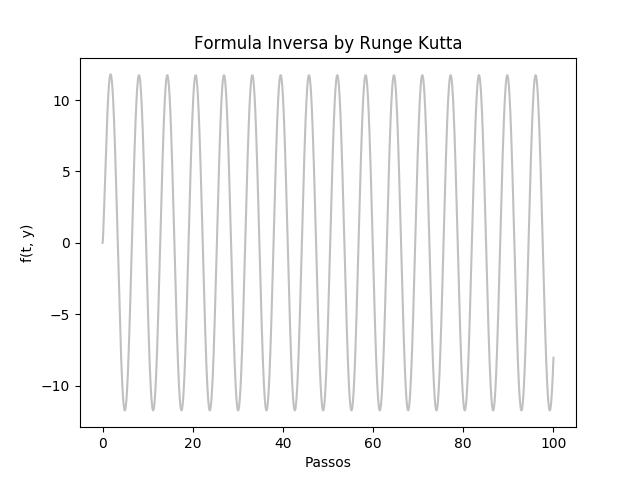
\includegraphics[width=.4\textwidth]{problemas/metodos_q3/circuito_inversa.png}
        \end{center}
        \caption{Métodos de passos simples para a equação da corrente i1}
    \end{figure}
    \begin{figure}[H]
        \begin{center}
            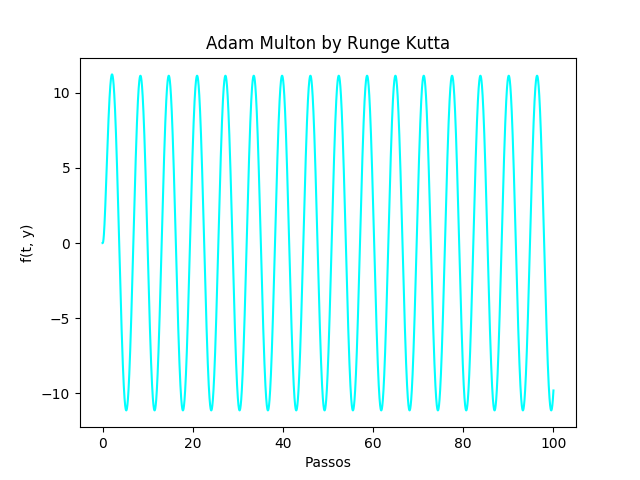
\includegraphics[width=.4\textwidth]{problemas/metodos_q3/circuito2_multon.png}
            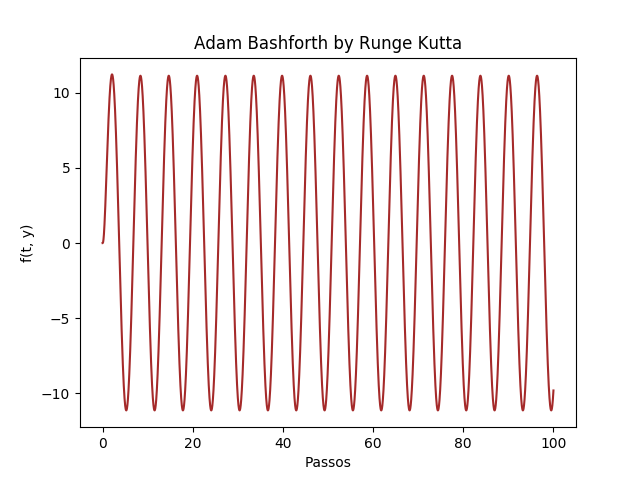
\includegraphics[width=.4\textwidth]{problemas/metodos_q3/circuito2_bashforth.png}
            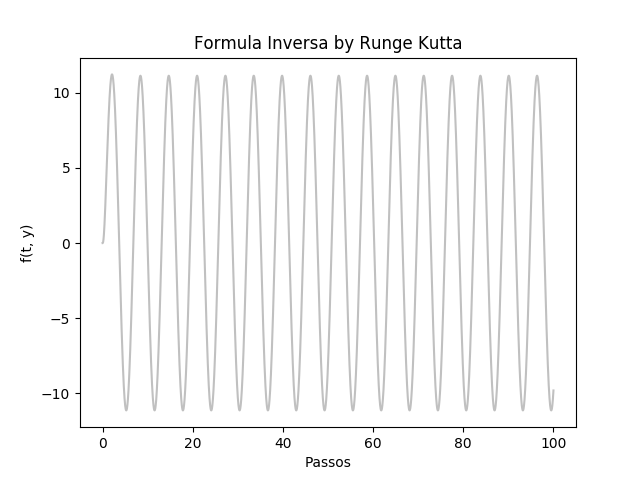
\includegraphics[width=.4\textwidth]{problemas/metodos_q3/circuito2_inversa.png}
        \end{center}
        \caption{Métodos de passos simples para a equação da corrente i2}
    \end{figure}
    
    Para obter o valor máximo e mínimo que as correntes podem atingir, podemos derivar a equação referente às correntes \(i_{1}\) e \(i_{2}\) e igualar a zero, de modo a obtermos o pico (amplitude), que é onde ocorre a corrente máxima e mínima.
    
    \begin{empheq}[left=\empheqlbrace]{align}
      i_{1}(t) &= 2e^{-2t} + \frac{18}{29}e^{-12t} + \frac{332}{29}\sin{t} - \frac{76}{29}\cos{t} \\
      i'_{1}(t) &= \frac{-216}{29}e^{-12t} - 4e^{-2t} + \frac{76}{29}\sin{t} + \frac{332}{29}\cos{t} = 0
    \end{empheq}
    
    \begin{empheq}[left=\empheqlbrace]{align}
      i_{2}(t) &= 6e^{-2t} - \frac{6}{29}e^{-12t} + \frac{276}{29}\sin{t} - \frac{168}{29}\cos{t} \\
      i'_{2}(t) &= \frac{72}{29}e^{-12t} - 12e^{-2t} + \frac{168}{29}\sin{t} + \frac{276}{29}\cos{t} = 0
    \end{empheq}
    
    Observando a derivada e rearranjando os termos, obtemos que as correntes máximas e seus respectivos tempos são:
    
    \begin{empheq}[left=\empheqlbrace]{align}
      i_{1_{max}} &= 11.74 A (t = 6.51)\\
      i_{2_{max}} &= 11.14 A (t = 6.83)
    \end{empheq}
    
    Analogamente, as correntes mínimas e seus respectivos tempos são:
    
    \begin{empheq}[left=\empheqlbrace]{align}
      i_{1_{min}} &= -11.74 A (t = 3.36)\\
      i_{2_{min}} &= -11.14 A (t = 3.68)
    \end{empheq}
    
\newpage
\end{document}